%%%%%%%% ICML 2026 EXAMPLE LATEX SUBMISSION FILE %%%%%%%%%%%%%%%%%

\documentclass{article}

% Recommended, but optional, packages for figures and better typesetting:
\usepackage{microtype}
\usepackage{graphicx}
\usepackage{subcaption}
\usepackage{booktabs} % for professional tables
\usepackage{stfloats}

% hyperref makes hyperlinks in the resulting PDF.
% If your build breaks (sometimes temporarily if a hyperlink spans a page)
% please comment out the following usepackage line and replace
% \usepackage{icml2026} with \usepackage[nohyperref]{icml2026} above.
\usepackage{hyperref}


% Attempt to make hyperref and algorithmic work together better:
% Use the following line for the initial blind version submitted for review:
% \usepackage{icml2026}

% For preprint, use
\usepackage[preprint]{icml2026}

% If accepted, instead use the following line for the camera-ready submission:
% \usepackage[accepted]{icml2026}

\usepackage{amsmath}
\usepackage{amssymb}
\usepackage{mathtools}
\usepackage{amsthm}


% if you use cleveref..
\usepackage[capitalize,noabbrev]{cleveref}

%%%%%%%%%%%%%%%%%%%%%%%%%%%%%%%%
% THEOREMS
%%%%%%%%%%%%%%%%%%%%%%%%%%%%%%%%
\theoremstyle{plain}
\newtheorem{theorem}{Theorem}[section]
\newtheorem{proposition}[theorem]{Proposition}
\newtheorem{lemma}[theorem]{Lemma}
\newtheorem{corollary}[theorem]{Corollary}
\theoremstyle{definition}
\newtheorem{definition}[theorem]{Definition}
\newtheorem{assumption}[theorem]{Assumption}
\theoremstyle{remark}
\newtheorem{remark}[theorem]{Remark}

% Todonotes is useful during development; simply uncomment the next line
%    and comment out the line below the next line to turn off comments
%\usepackage[disable,textsize=tiny]{todonotes}
\usepackage[textsize=tiny]{todonotes}

% The \icmltitle you define below is probably too long as a header.
% Therefore, a short form for the running title is supplied here:
\icmltitlerunning{AskBeforeAnswer: Aligning Language Agents with Programmatic RL}

\begin{document}

\twocolumn[
  \icmltitle{AskBeforeAnswer: Aligning Large Language Models for \\
  Ambiguity Resolution via Group Relative Policy Optimization}

  % It is OKAY to include author information, even for blind submissions: the
  % style file will automatically remove it for you unless you've provided
  % the [accepted] option to the icml2026 package.

  % List of affiliations: The first argument should be a (short) identifier you
  % will use later to specify author affiliations Academic affiliations
  % should list Department, University, City, Region, Country Industry
  % affiliations should list Company, City, Region, Country

  % You can specify symbols, otherwise they are numbered in order. Ideally, you
  % should not use this facility. Affiliations will be numbered in order of
  % appearance and this is the preferred way.
  \icmlsetsymbol{equal}{*}

  \begin{icmlauthorlist}
    \icmlauthor{Christian Contreras Campana}{ind}
  \end{icmlauthorlist}

  \icmlaffiliation{ind}{Independent Researcher}

  \icmlcorrespondingauthor{Christian Contreras Campana}{chrisjcc.physics@gmail.com}

  % You may provide any keywords that you find helpful for describing your
  % paper; these are used to populate the "keywords" metadata in the PDF but
  % will not be shown in the document
  \icmlkeywords{Machine Learning, ICML}

  \vskip 0.3in
]

% this must go after the closing bracket ] following \twocolumn[ ...

% This command actually creates the footnote in the first column listing the
% affiliations and the copyright notice. The command takes one argument, which
% is text to display at the start of the footnote. The \icmlEqualContribution
% command is standard text for equal contribution. Remove it (just {}) if you
% do not need this facility.

% Use ONE of the following lines. DO NOT remove the command.
% If you have no special notice, KEEP empty braces:
\printAffiliationsAndNotice{}  % no special notice (required even if empty)
% Or, if applicable, use the standard equal contribution text:
% \printAffiliationsAndNotice{\icmlEqualContribution}

\begin{abstract}
While large language models (LLMs) demonstrate impressive reasoning capabilities, they frequently struggle with ambiguous or underspecified queries, often hallucinating answers or guessing user intent. A robust conversational agent must reliably navigate the ``clarify-or-act'' decision boundary, detecting ambiguity and asking targeted clarification questions before proceeding. In this work, we introduce AskBeforeAnswer, a novel training framework that aligns LLMs to a clarification-first behavior. Rather than relying solely on standard Supervised Fine-Tuning (SFT) which is prone to hallucination, we propose a two-stage hybrid pipeline utilizing Group Relative Policy Optimization (GRPO) warm-started from an SFT foundation. Our methodology uses purely programmatic, deterministic reward functions during the GRPO stage to explicitly penalize hallucination and enforce logical action routing. Empirical evaluations demonstrate a fundamental trade-off between post-training paradigms: DPO excels at stylistic alignment and balancing clarify ratios, while GRPO excels at factual calibration and safety. Our SFT$\rightarrow$GRPO pipeline achieves flawless 100\% schema adherence while doubling factual accuracy over SFT baselines, establishing a highly conservative, hallucination-resistant agent.
\end{abstract}

\section{Introduction}

The widespread deployment of large language models (LLMs) in conversational and instruction-following contexts has revolutionized human-computer interaction. While these models demonstrate impressive linguistic fluency and reasoning capabilities, they fundamentally struggle with a critical human-like skill: handling ambiguous or underspecified instructions. Current systems often assume perfect input and are poorly equipped to deal with the inherent uncertainty present in real-world human communication. 

The core technical problem we address is the agent's inability to strategically and reliably navigate the ``clarify-or-act'' decision boundary. When a user request is ambiguous, an agent must determine whether it has sufficient information to act or whether clarification is necessary to avoid incorrect or suboptimal actions. An agent that consistently acts on incorrect assumptions erodes user trust, while one that over-clarifies introduces unnecessary friction.

Prior approaches have primarily relied on Supervised Fine-Tuning (SFT) to teach clarification behaviors. However, SFT suffers from imitation errors; models learn to mimic the surface-level structure of training data without causally understanding the underlying rules. In this work, we introduce a novel alignment framework that explores the distinct impacts of Direct Preference Optimization (DPO) versus Group Relative Policy Optimization (GRPO) when warm-started from an SFT foundation. By utilizing purely programmatic, deterministic reward functions to penalize logical errors and hallucinations during online rollouts, our SFT$\rightarrow$GRPO pipeline establishes a highly calibrated, cautious agent. We demonstrate that while DPO effectively aligns the stylistic nuance of clarifications, GRPO is necessary to explicitly optimize factual accuracy and safety on the clarify-or-act problem.

\section{Related Work}

Prior work on ambiguity handling in language agents spans several directions, including clarification question generation, ambiguity prediction, multi-turn reasoning, and uncertainty-aware decision making. 

\textbf{Supervised Clarification:} Recent frameworks, such as \emph{Learning to Clarify}, propose contrastive self-training pipelines where models learn to ask clarification questions that improve downstream performance. While these works demonstrate that LLMs can learn helpful clarification behaviors, they typically treat ambiguity as a single undifferentiated phenomenon and rely purely on behavioral cloning, making them brittle to out-of-distribution formatting failures.

\textbf{Reinforcement Learning for Ambiguity:} Another closely related line of research is SWEET-RL, which studies the clarify-or-act decision as a reinforcement learning problem over multi-turn interactions. Although effective, SWEET-RL relies heavily on reward shaping and emergent behaviors, which do not provide an interpretable grounding of \emph{why} a query is ambiguous. STaR-GATE similarly examines taxonomy-guided prompting but does not integrate ambiguity classification with strategy selection using direct policy optimization.

Our approach differs fundamentally by anchoring the clarify-or-act decision directly to extracted \emph{facets} (missing informational parameters) and enforcing strict structural adherence through programmatic GRPO reward functions, effectively eliminating the need for an LLM-as-a-judge during the initial structural alignment phase.

\section{Preliminaries \& Mathematical Formulation}
To model dialogue state routing under query ambiguity, we reframe the alignment problem from standard next-token sequence generation to an online routing optimization problem.

\subsection{Token-Level Schema Constraint}
Let $x \sim \mathcal{D}$ represent an initial user prompt. We force the language policy $\pi_\theta$ to output responses conforming strictly to a structured, four-tiered programmatic schema:
$$y = [\,\text{Action:}\, a, \;\text{Reasoning:}\, r, \;\text{Facets:}\, f, \;\text{Response:}\, s\,]$$ 
where:
\begin{itemize}
\item $a \in \{\text{Clarify}, \text{Answer}\}$ represents the routing action decision.
\item $r$ is the chain-of-thought rationale justifying the action selection.
\item $f = [f_1, f_2, \dots, f_k]$ is a generated list of missing informational parameters (or Facets), which must be non-empty if and only if $a = \text{Clarify}$.
\item $s$ is the final text payload delivered to the user (either a clarifying question or the terminal answer).
\end{itemize}

\subsection{Reference Baselines: SFT, DPO, and ORPO}

\textbf{Supervised Fine-Tuning (SFT):} Our behavioral cloning phase optimizes the standard cross-entropy loss over a curated corpus $\mathcal{D}_{\text{SFT}}$ of gold-standard routing structures:
$$\mathcal{L}_{\text{SFT}}(\theta) = -\mathbb{E}_{(x,y) \sim \mathcal{D}_{\text{SFT}}} \left[ \sum_{t=1}^{\vert y \vert} \log \pi_\theta(y_t \mid x, y_{<t}) \right]$$ 

\textbf{Direct Preference Optimization (DPO):} Given paired preference data $\mathcal{D}_{\text{pref}} = \{(x, y_w, y_l)\}$, where $y_w$ represents a response with correct ambiguity resolution and formatting, and $y_l$ contains errors (e.g., over-clarification or hallucinated answering), the objective is:
%$$\mathcal{L}_{\text{DPO}}(\theta; \pi_{\text{ref}}) = -\mathbb{E}_{(x, y_w, y_l) \sim \mathcal{D}_{\text{pref}}} \left[ \log \sigma \left( \beta \log \frac{\pi_\theta(y_w \mid x)}{\pi_{\text{ref}}(y_w \mid x)} - \beta \log \frac{\pi_\theta(y_l \mid x)}{\pi_{\text{ref}}(y_l \mid x)} \right) \right]$$
\begin{align}
\Delta_\theta
&=
\log \frac{\pi_\theta(y_w \mid x)}
{\pi_{\text{ref}}(y_w \mid x)}
-
\log \frac{\pi_\theta(y_l \mid x)}
{\pi_{\text{ref}}(y_l \mid x)}
\\
\mathcal{L}_{\text{DPO}}(\theta; \pi_{\text{ref}})
&=
-\mathbb{E}_{(x, y_w, y_l) \sim \mathcal{D}_{\text{pref}}}
\left[
\log \sigma(\beta \Delta_\theta)
\right]
\end{align}

\textbf{Odds Ratio Preference Optimization (ORPO):} To evaluate single-stage alignment without a reference policy, we implement ORPO as an alternative baseline:
%$$\mathcal{L}_{\text{ORPO}}(\theta) = \mathcal{L}_{\text{SFT}}(\theta) - \lambda \cdot \mathbb{E}_{(x, y_w, y_l) \sim \mathcal{D}_{\text{pref}}} \left[ \log \sigma \left( \log \frac{\pi_\theta(y_w \mid x)}{1 - \pi_\theta(y_w \mid x)} - \log \frac{\pi_\theta(y_l \mid x)}{1 - \pi_\theta(y_l \mid x)} \right) \right]$$
\begin{align}
\Delta_{\text{odds}}
&=
\log \frac{\pi_\theta(y_w \mid x)}
{1 - \pi_\theta(y_w \mid x)}
-
\log \frac{\pi_\theta(y_l \mid x)}
{1 - \pi_\theta(y_l \mid x)}
\\
\mathcal{L}_{\text{ORPO}}(\theta)
&=
\mathcal{L}_{\text{SFT}}(\theta)
-
\lambda \cdot
\mathbb{E}_{(x, y_w, y_l) \sim \mathcal{D}_{\text{pref}}}
\left[
\log \sigma \left(
\Delta_\theta^{\text{OR}}
\right)
\right]
\end{align}

\section{Dataset Construction and Curation}
\label{sec:dataset}
To train and evaluate the clarify-or-act policy, we construct a specialized dataset derived from the open-source AmbigNQ corpus \cite{min2020ambigqa}. The original dataset contains open-domain questions with multiple plausible interpretations, making it an ideal testbed for ambiguity resolution. However, standard supervised datasets often induce mode collapse during fine-tuning, where the model exploits the majority class (e.g., learning to answer everything and forgetting to ask for clarification). To prevent this, we developed a rigorous data curation and synthetic generation pipeline.

\textbf{Synthetic Augmentation:} We employ a lightweight instructor model (Qwen 2.5 7B Instruct) to dynamically generate deep structural elements for each training example. The model generates a Chain-of-Thought \emph{Reasoning} block to justify its actions, and extracts missing informational \emph{Facets} when a question is ambiguous. 

\textbf{Class Balancing and Strict Filtering:} To guarantee a balanced policy, the dataset is dynamically undersampled to enforce a strict 50/50 split between \emph{Clarify} and \emph{Answer} actions. Furthermore, we apply strict row filtering to discard generated examples where the synthetic LLM hallucinated conflicting labels (e.g., classifying a query as an ``Answer'' while simultaneously generating disambiguating facets).

\textbf{Contrastive Hard Negatives:} For preference optimization (DPO), we require paired chosen and rejected responses. Instead of using trivial rejected responses (e.g., ``I don't know''), we synthesize highly plausible \emph{Hard Negatives}. For instance, if the ground truth action is to clarify, the rejected response is forced to be a confident, un-disambiguated direct answer. Conversely, clear questions are paired with rejected responses that unnecessarily ask for clarification. This forces the preference algorithm to learn true semantic boundaries rather than memorizing trivial rejection templates.

\section{Methodology: The Clarify-or-Act Ablation Suite}
Our core contribution evaluates online, critic-free reinforcement learning using Group Relative Policy Optimization (GRPO) as a direct substitute or prelude to preference optimization stages.

\subsection{Group Relative Policy Optimization (GRPO) Base}
For each prompt $x$, we sample a group of outputs $\{y_1, y_2, \dots, y_G\}$ from the current policy $\pi_\theta$. GRPO optimizes the policy by computing relative advantages across the sampled group instead of utilizing a separate value network:
%$$\mathcal{L}_{\text{GRPO}}(\theta) = -\frac{1}{G} \sum_{i=1}^G \left[ \min \left( \frac{\pi_\theta(y_i \mid x)}{\pi_{\text{old}}(y_i \mid x)} A_i, \text{clip}\left(\frac{\pi_\theta(y_i \mid x)}{\pi_{\text{old}}(y_i \mid x)}, 1-\epsilon, 1+\epsilon\right) A_i \right) - \beta \mathbb{D}_{\text{KL}}(\pi_\theta \parallel \pi_{\text{ref}}) \right]$$ 
\begin{align}
r_i(\theta)
&=
\frac{\pi_\theta(y_i \mid x)}
{\pi_{\text{old}}(y_i \mid x)}
\\
\hat{r}_i(\theta)
&=
\mathrm{clip}\!\left(
r_i(\theta),
1-\epsilon,
1+\epsilon
\right)
\\
\mathcal{L}_{\text{GRPO}}(\theta)
&=
-\frac{1}{G}
\sum_{i=1}^G
\min \Big(
r_i(\theta) A_i,
\hat{r}_i(\theta) A_i
\Big)
\\
&\quad
+ \beta \,
\mathbb{D}_{\mathrm{KL}}\!\left(
\pi_\theta \,\|\, \pi_{\text{ref}}
\right)
\end{align}
The group relative advantage $A_i$ is computed by standardizing the programmatic rewards:
$$A_i = \frac{\mathcal{R}(x, y_i) - \frac{1}{G}\sum_{j=1}^G \mathcal{R}(x, y_j)}{\text{std}(\mathcal{R}(x, y_1), \dots, \mathcal{R}(x, y_G))}$$ 

\subsection{Alternative Loss Formulations}
To systematically test distribution robustness and sample efficiency, our suite implements configuration switches for two advanced modifications:
\begin{itemize}
\item \textbf{DAPO:} Modifies GRPO by decoupling the clipping mechanics between token-level probabilities and value expectations, while dynamically altering sample size $G$ based on training iteration variance to speed up convergence. 
\item \textbf{Dr. GRPO (Distributionally Robust GRPO):} Adapts the framework of Distributionally Robust Optimization (DRO) to manage heterogeneous prompt distributions. Rather than maximizing average group performance, Dr. GRPO constructs an ambiguity set $\mathcal{P}$ around the nominal prompt distribution and optimizes against the worst-case difficulty stratum:
$$\min_\theta \max_{P \in \mathcal{P}} \mathbb{E}_{x \sim P} \left[ \mathcal{L}_{\text{GRPO}}(\theta; x) \right]$$ 
\end{itemize}

\subsection{Deterministic Programmatic Reward Function}
The reward function $\mathcal{R}(x, y)$ is calculated entirely via deterministic Python validation scripts. It is a linear combination of four sub-rewards:
%$$\mathcal{R}(x, y) = \omega_1 \mathcal{R}_{\text{format}}(y) + \omega_2 \mathcal{R}_{\text{routing}}(x, a) + \omega_3 \mathcal{R}_{\text{facet}}(x, f) + \omega_4 \mathcal{R}_{\text{len}}(y)$$ 
\begin{align}
\mathcal{R}(x, y)
&=
\sum_{k=1}^{4} \omega_k \mathcal{R}_k(x, y)
\end{align}

\begin{align}
\mathcal{R}_1 &= \mathcal{R}_{\text{format}}(y), \quad
\mathcal{R}_2 = \mathcal{R}_{\text{routing}}(x, a), \\
\mathcal{R}_3 &= \mathcal{R}_{\text{facet}}(x, f), \quad
\mathcal{R}_4 = \mathcal{R}_{\text{len}}(y)
\end{align}

%\begin{figure}[ht]
%\begin{center}
%\begin{verbatim}
%+------------------------------------------------------------------------+
%|                        Reward Execution Engine                         |
%+------------------------------------------------------------------------+
%                                    |
%                                    v
%       +----------------------------------------------------------+
%       |             Format Check: R_format(y)                    |
%       |    Validates schema blocks via regex/JSON parser         |
%       +----------------------------+-----------------------------+
%                                    |
%                  +-----------------+-----------------+
%                  v Pass                              v Fail (-1.0)
%+----------------------------------+        +----------------------------+
%|    Routing Check: R_routing      |        | Terminate Early            |
%| Compares action 'a' with ground  |        | Skip downstream processing |
%| truth data annotation            |        +----------------------------+
%+-----------------+----------------+
%                  |
%                  v Pass
%+----------------------------------+
%|     Facet Validation: R_facet    |
%| If Clarify: measures string match|
%| or exact parameter key matching  |
%+-----------------+----------------+
%                  |
%                  v Pass
%+----------------------------------+
%|     Length Penalty: R_len        |
%| Penalizes verbose outputs using  |
%| a dynamic length scaling term    |
%+----------------------------------+
%\end{verbatim}
%\caption{The Deterministic Programmatic Reward pipeline for GRPO.}
%\end{center}
%\end{figure}

\begin{figure}[t]
\centering
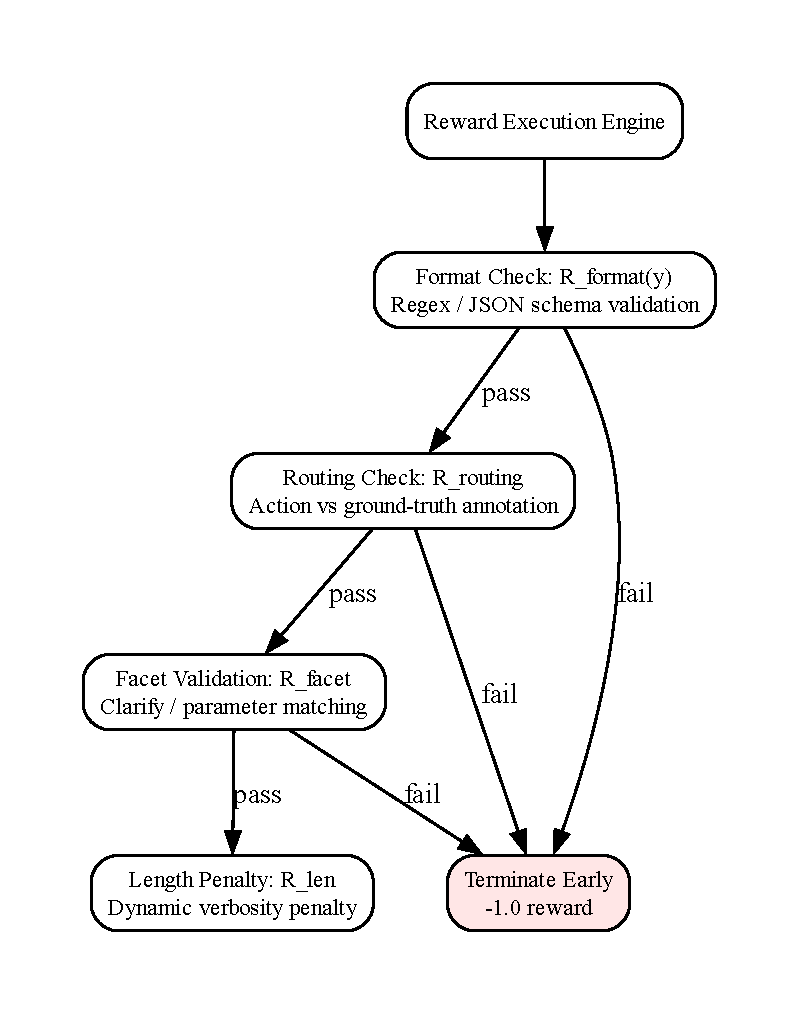
\includegraphics[width=\linewidth]{figures/grpo_reward_pipeline.pdf}
\caption{Deterministic programmatic reward pipeline used in GRPO.}
\label{fig:reward_pipeline}
\end{figure}

\section{Empirical Evaluation \& Pipeline Comparisons}
For a detailed analysis of optimization stability, sample efficiency, and training/validation loss curves across our ablation suite, we direct the reader to Appendix \ref{sec:training_details}.

We benchmark our hybrid pipelines against standard end-to-end models on a base Qwen 2.5 7B architecture using the AmbigNQ dataset. Our primary comparisons are between the classic $\text{SFT} \rightarrow \text{DPO}$ pipeline and our proposed $\text{GRPO} \rightarrow \text{DPO}$ approach.

\subsection{Evaluation Metrics}
To fully capture the nuances of the clarify-or-act problem, we evaluate the models using 9 core metrics across deterministic structural scoring and LLM-as-a-judge evaluations:
\begin{enumerate}
\item \textbf{Action Accuracy (Macro Accuracy):} The overall percentage of times the model correctly predicts the target action (Clarify vs. Answer).
\item \textbf{Clarify Detection (Precision/Recall/F1):} Treats ``Clarify'' as the positive class, evaluating if the model correctly identified ambiguous questions without hallucinating ambiguity.
\item \textbf{Clarify F1:} The harmonic mean of Clarify Precision and Clarify Recall.
\item \textbf{Action F1 (Answer Class):} Evaluates policy action selection rather than text quality. Treats ``Answer'' as the positive class. Penalizes the model for refusing to answer a straightforward question or for confidently answering a question that it should have clarified.
\item \textbf{Macro F1:} The unweighted mathematical average of Clarify F1 and Action F1 (Answer Class).
\item \textbf{Answer Accuracy:} Evaluated only on ground-truth Answer cases, measuring whether the generated answer semantically matches the target answer using fuzzy token-matching.
\item \textbf{Clarify Ratio:} The total number of predicted Clarify actions divided by the total number of ground-truth Clarify actions, indicating bias toward over- or under-clarifying.
\item \textbf{Facet Generation Rate:} The percentage of predicted Clarify actions that successfully included a non-empty list of extracted facets.
\item \textbf{LLM-as-a-Judge Quality Metrics:} Ambiguity Detection F1, Clarification Quality F1, and Clarification Usefulness, scored subjectively by a strong teacher model.
\end{enumerate}

\subsection{Main Alignment Results}
Table \ref{tab:main_results} illustrates the performance of our ablation suite, showcasing a direct showdown between standard behavioral cloning (SFT), preference optimization (SFT $\rightarrow$ DPO), and online reinforcement learning (SFT $\rightarrow$ GRPO). The SFT warm-start completely cured the catastrophic mode collapse previously observed in GRPO-only runs, allowing all post-trained pipelines to achieve a flawless 100\% Facet Generation Rate (FGR).

\begin{table*}[!ht]
  \caption{Main Alignment Results: The clarify-or-act showdown comparing behavioral cloning (SFT) against preference (DPO) and reward (GRPO) optimization.}
  \label{tab:main_results}
  \begin{center}
    \begin{small}
      \begin{sc}
        \begin{tabular}{lccccccc}
          \toprule
          Pipeline & Act-Acc & C-F1 & Ans-F1 & Macro F1 & C-Ratio & Ans-Acc & FGR \\
          \midrule
          Base & 62.0\% & 75.3\% & 17.4\% & 46.4\% & 1.57 & 5.0\% & 8.5\% \\
          SFT & 64.0\% & 73.5\% & 43.8\% & \textbf{58.6\%} & 1.27 & 5.0\% & \textbf{100\%} \\
          SFT $\rightarrow$ DPO & 62.0\% & 70.8\% & \textbf{45.7\%} & 58.2\% & \textbf{1.17} & 0.0\% & \textbf{100\%} \\
          SFT $\rightarrow$ GRPO & \textbf{64.0\%} & \textbf{75.0\%} & 35.7\% & 55.4\% & 1.40 & \textbf{10.0\%} & \textbf{100\%} \\
          \bottomrule
        \end{tabular}
      \end{sc}
    \end{small}
  \end{center}
\end{table*}

\subsection{Discussion: Style vs. Logic Calibration}
The results highlight a fundamental divergence in agent personalities depending on the Stage 2 optimization algorithm. 

\textbf{DPO for Stylistic Alignment:} The SFT $\rightarrow$ DPO pipeline excels at refining the stylistic nuance of the policy. By leveraging generative hard negatives, DPO successfully mitigated over-clarification, dropping the Clarify Ratio to a near-ideal 1.17 and boosting Action F1 (Answer Class) to 45.7\%. However, it failed to improve factual retrieval, suffering from complete hallucination on closed-book questions (0\% Answer Accuracy).

\textbf{GRPO for Factual Calibration:} Conversely, the SFT $\rightarrow$ GRPO pipeline leveraged the \texttt{accuracy\_reward\_func} to double the factual Answer Accuracy (10.0\% vs 5.0\% for SFT). Because the reward heavily penalizes hallucinations, GRPO learned a highly calibrated, cautious policy. Answering is deemed ``risky,'' causing the model to clarify more often to avoid penalties (increasing Clarify Ratio to 1.40 and pulling Action F1 down to 35.7\%). This demonstrates that online RL with deterministic rewards is highly effective at enforcing factual logic and safety, while DPO is better suited for tone and formatting alignment.

\subsection{Ablation Studies \& Extended Baselines}
To further contextualize the performance of our primary pipelines, we conducted extended ablation studies evaluating the necessity of the SFT warm-start and the efficacy of single-stage optimization (see Appendix \ref{sec:appendix_full_eval} for the comprehensive evaluation leaderboard across all 12 metrics).

\textbf{The Failure of Preference Optimization without an SFT Prior:}
Running DPO directly on the base model (\texttt{dpo\_only}) results in catastrophic structural collapse, yielding an abysmal Macro F1 of 41.7\% and a Facet Generation Rate of 8.3\%. This mathematically demonstrates that preference optimization is strictly a stylistic polisher; it is incapable of teaching structural schema or complex logic from scratch and requires a strong behavioral prior (SFT).

\textbf{The Merits of Single-Stage ORPO:}
As a single-stage algorithm, ORPO performs admirably without a dedicated SFT warm-up, achieving a 93.2\% Facet Generation Rate and a 53.2\% Macro F1. While it is highly efficient, it slightly underperforms the dedicated two-stage SFT $\rightarrow$ DPO pipeline (100\% FGR, 58.2\% Macro F1), suggesting that for highly complex structural tasks, explicitly separating behavioral cloning from preference alignment yields more robust results.

\textbf{Preserving Semantic Safety (LLM-as-a-Judge):}
Across all post-trained models (SFT, DPO, GRPO), qualitative metrics such as Clarification Quality ($\sim$79.6\%) and Usefulness ($\sim$89.8\%) remain remarkably high. This proves that forcing the model to adhere to a strict programmatic schema does not degrade the natural language quality or helpfulness of its responses; semantic nuance is preserved while logical safety is vastly improved.

\section{Conclusion}
In this work, we presented AskBeforeAnswer, an alignment framework that effectively teaches language agents to safely navigate the clarify-or-act decision boundary. We demonstrated a critical divergence in post-training optimization: DPO excels at aligning the stylistic nuance and distribution of actions, whereas GRPO, when warm-started from an SFT foundation and guided by deterministic rewards, excels at factual calibration. Our SFT$\rightarrow$GRPO pipeline successfully doubled factual accuracy and eliminated mode collapse, yielding a highly cautious, hallucination-resistant agent. We hope this work inspires future research into combining the formatting priors of SFT with the logical rigor of online RL to build safer, more reliable conversational AI.

\section{Limitations}
While our programmatic GRPO approach enforces strict structural compliance, the current reward formulations for facet generation ($\mathcal{R}_{\text{facet}}$) rely on relatively simple heuristics (e.g., regex matching and JSON parsing). They do not semantically evaluate whether the generated facets are genuinely useful for disambiguating the query, only that they are structurally present. Future work should investigate integrating an LLM-as-a-Judge or a fast local Reward Model directly into the GRPO step to provide graded, semantic rewards for facet quality.

\section*{Impact Statement}
This paper presents work whose goal is to advance the field of Machine Learning by improving the reliability and safety of conversational agents. By training models to ask clarification questions instead of hallucinating answers, we aim to reduce the spread of misinformation and increase user trust in AI systems. We do not foresee significant negative societal consequences arising directly from this work.

% In the unusual situation where you want a paper to appear in the
% references without citing it in the main text, use \nocite
\nocite{langley00}

\bibliography{main}
\bibliographystyle{icml2026}

%%%%%%%%%%%%%%%%%%%%%%%%%%%%%%%%%%%%%%%%%%%%%%%%%%%%%%%%%%%%%%%%%%%%%%%%%%%%%%%
%%%%%%%%%%%%%%%%%%%%%%%%%%%%%%%%%%%%%%%%%%%%%%%%%%%%%%%%%%%%%%%%%%%%%%%%%%%%%%%
% APPENDIX
%%%%%%%%%%%%%%%%%%%%%%%%%%%%%%%%%%%%%%%%%%%%%%%%%%%%%%%%%%%%%%%%%%%%%%%%%%%%%%%
%%%%%%%%%%%%%%%%%%%%%%%%%%%%%%%%%%%%%%%%%%%%%%%%%%%%%%%%%%%%%%%%%%%%%%%%%%%%%%%
\newpage
\appendix
\onecolumn
\section{Appendix: Training Details}
\label{sec:training_details}

In this section, we report the training dynamics to demonstrate optimization stability, convergence speed, and generalization without overfitting. The following plots are preliminary (as we plan to rerun the entire ablation suite) but illustrate the current training behavior for SFT and DPO:

\begin{itemize}
    \item \textbf{Training \& Evaluation Loss:} Demonstrates the convergence speed and stability of the loss across training stages (Figure \ref{fig:loss_comparisons}).
    \item \textbf{DPO Training Metrics:} Detailed metrics from the DPO stage including reward margins, log probabilities for chosen versus rejected responses, and classification accuracies (Figure \ref{fig:dpo_details}).
    \item \textbf{GRPO Training Metrics:} Illustrates the convergence of the programmatic reward and the KL divergence penalty during the reinforcement learning stage (Figure \ref{fig:grpo_details}).
\end{itemize}

\begin{figure}[htbp]
\centering
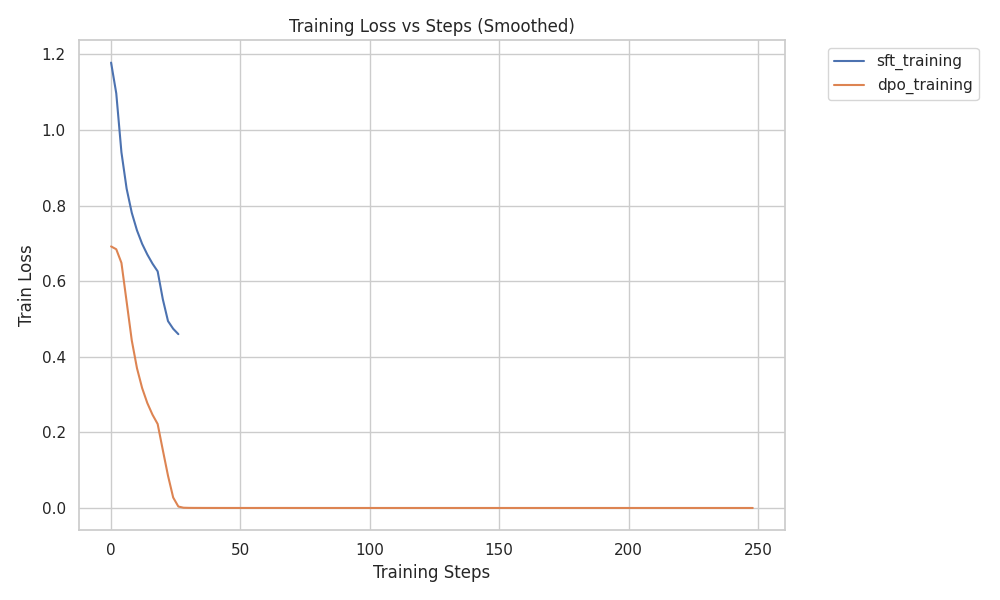
\includegraphics[width=0.48\textwidth]{figures/train_loss_comparison.png}
\hfill
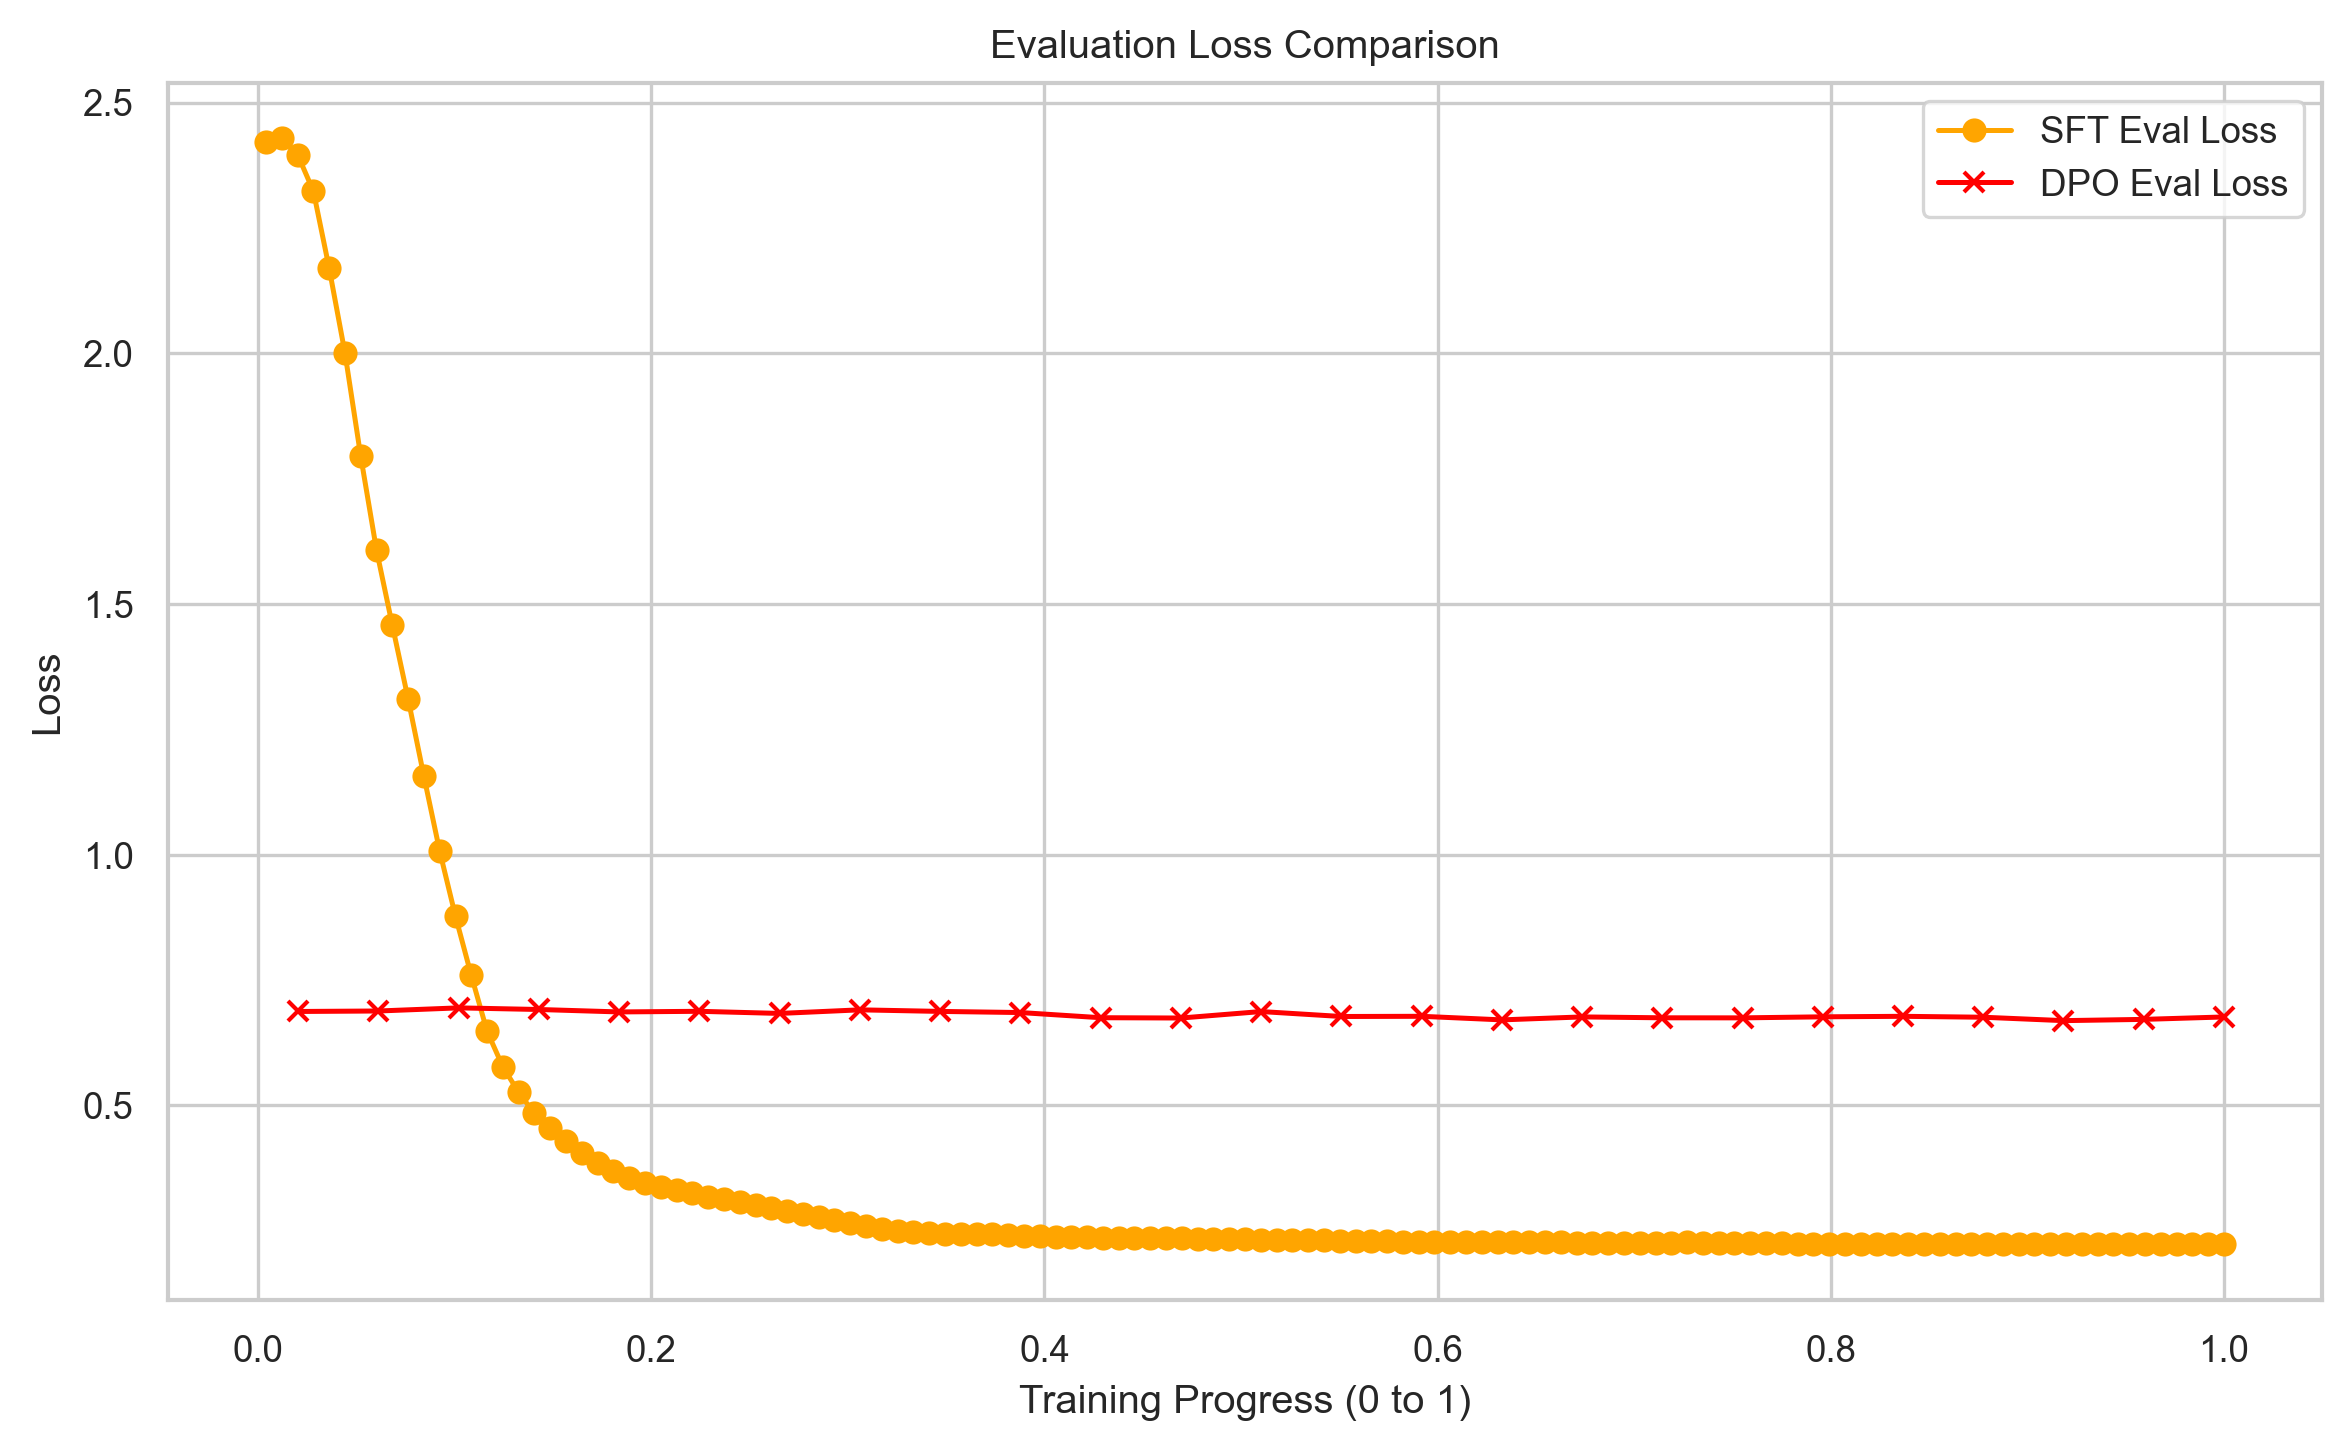
\includegraphics[width=0.48\textwidth]{figures/eval_loss_comparison.png}
\caption{Training (left) and Evaluation (right) loss curves comparing the ablation variants.}
\label{fig:loss_comparisons}
\end{figure}

\begin{figure}[htbp]
\centering

\includegraphics[width=0.32\textwidth]{figures/dpo_margin.png}
\hfill
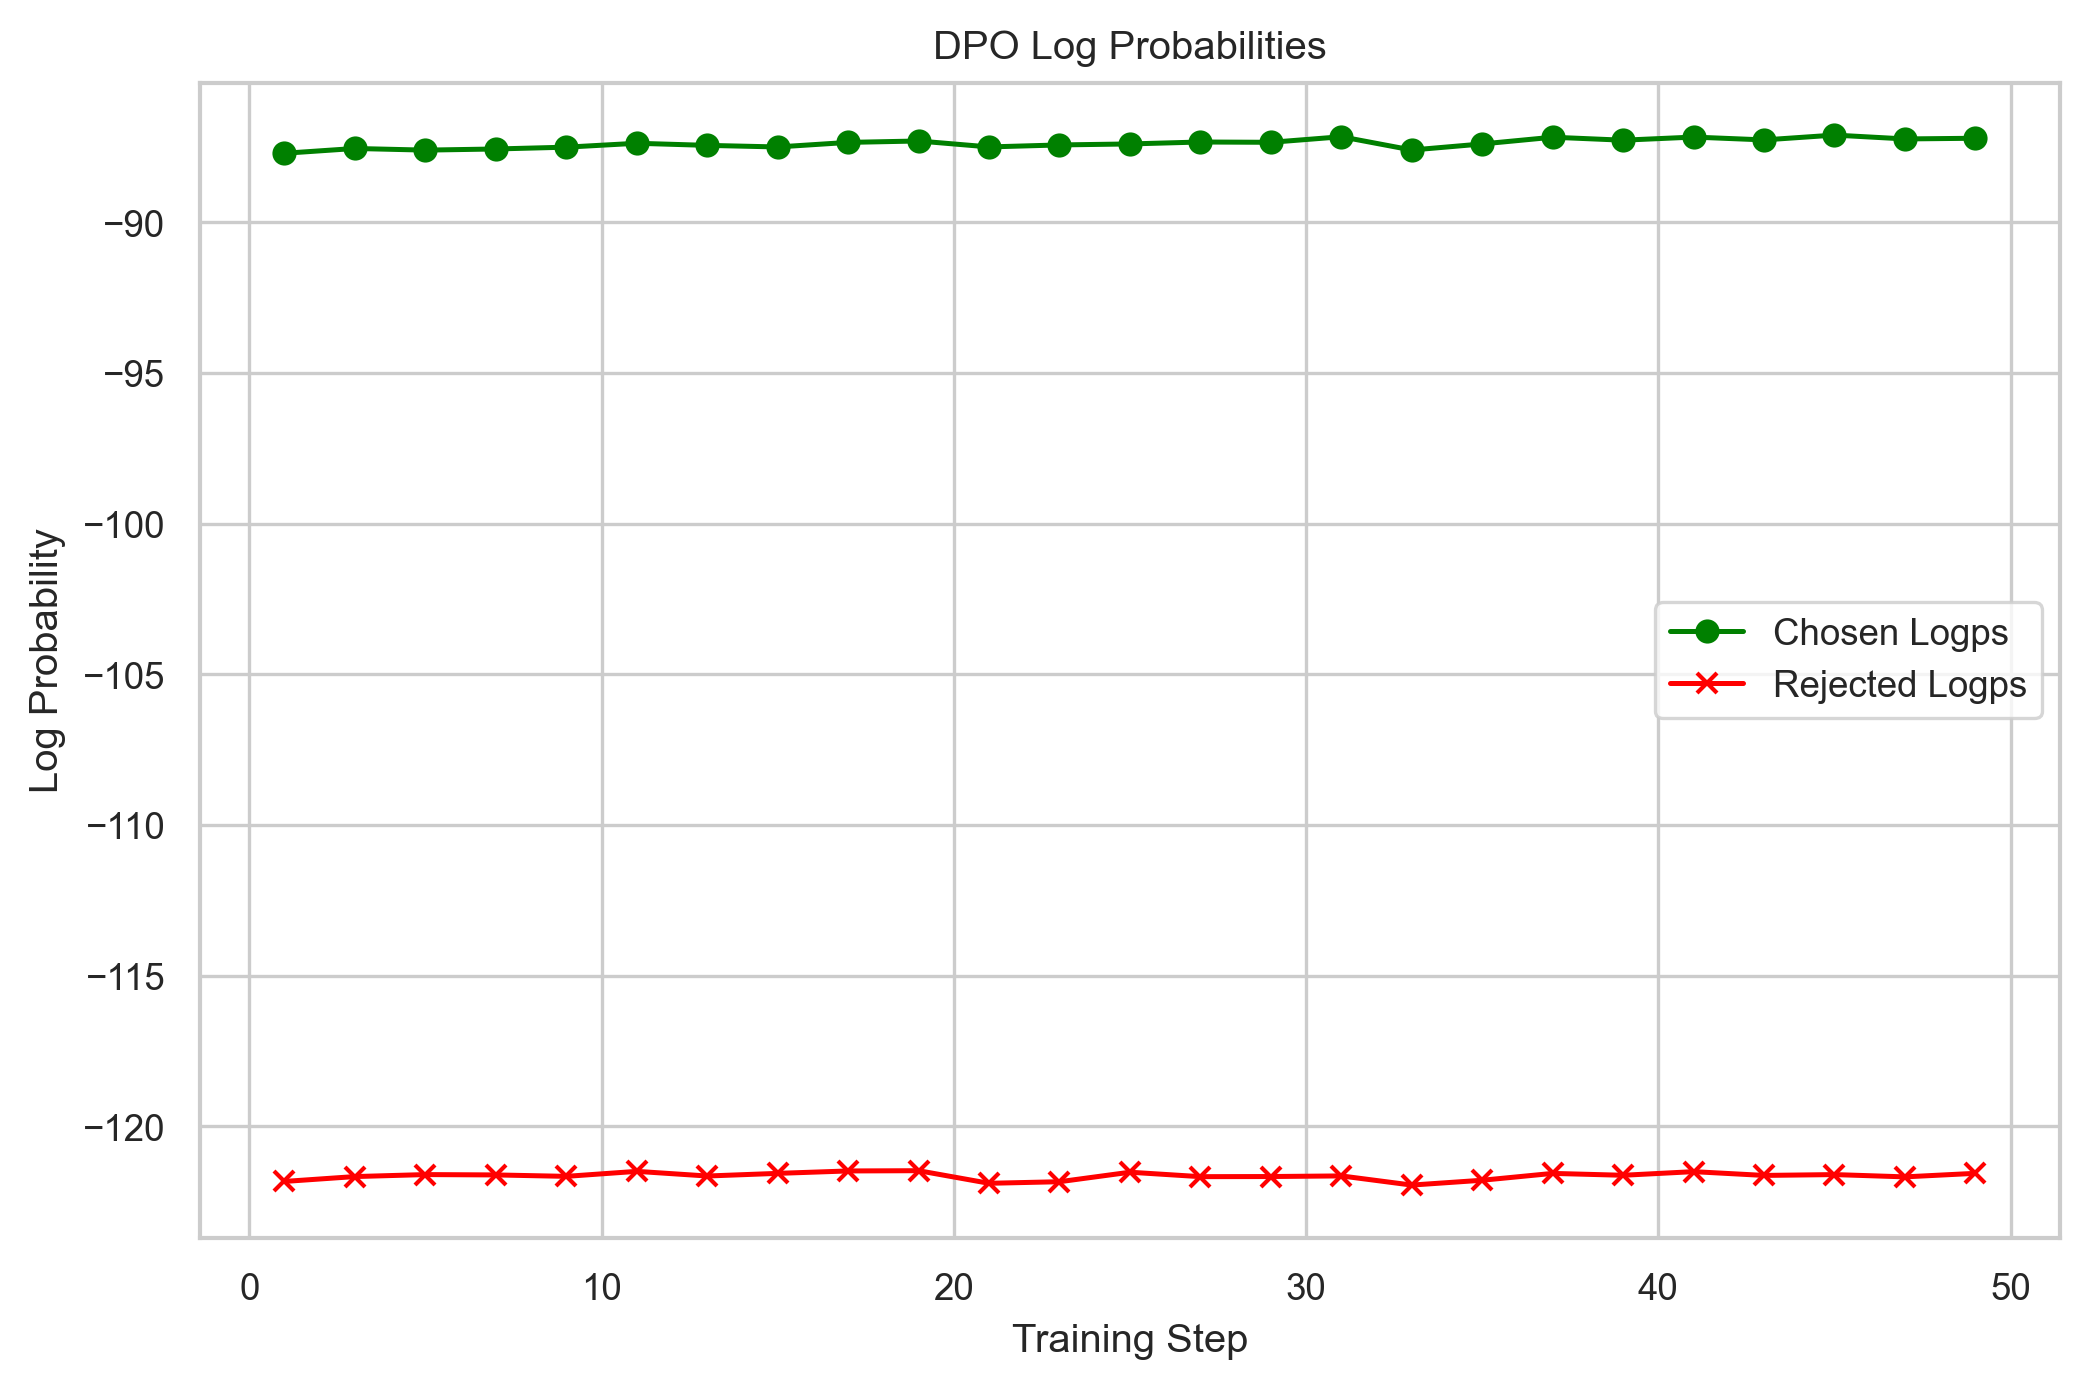
\includegraphics[width=0.32\textwidth]{figures/dpo_logprobs.png}
\hfill

\includegraphics[width=0.32\textwidth]{figures/dpo_accuracies.png}
\caption{Detailed DPO training metrics: Reward Margins (left), Log Probabilities (center), and Accuracies (right).}
\label{fig:dpo_details}
\end{figure}

\begin{figure}[htbp]
\centering

\includegraphics[width=0.48\textwidth]{figures/reward_convergence.png}
\hfill
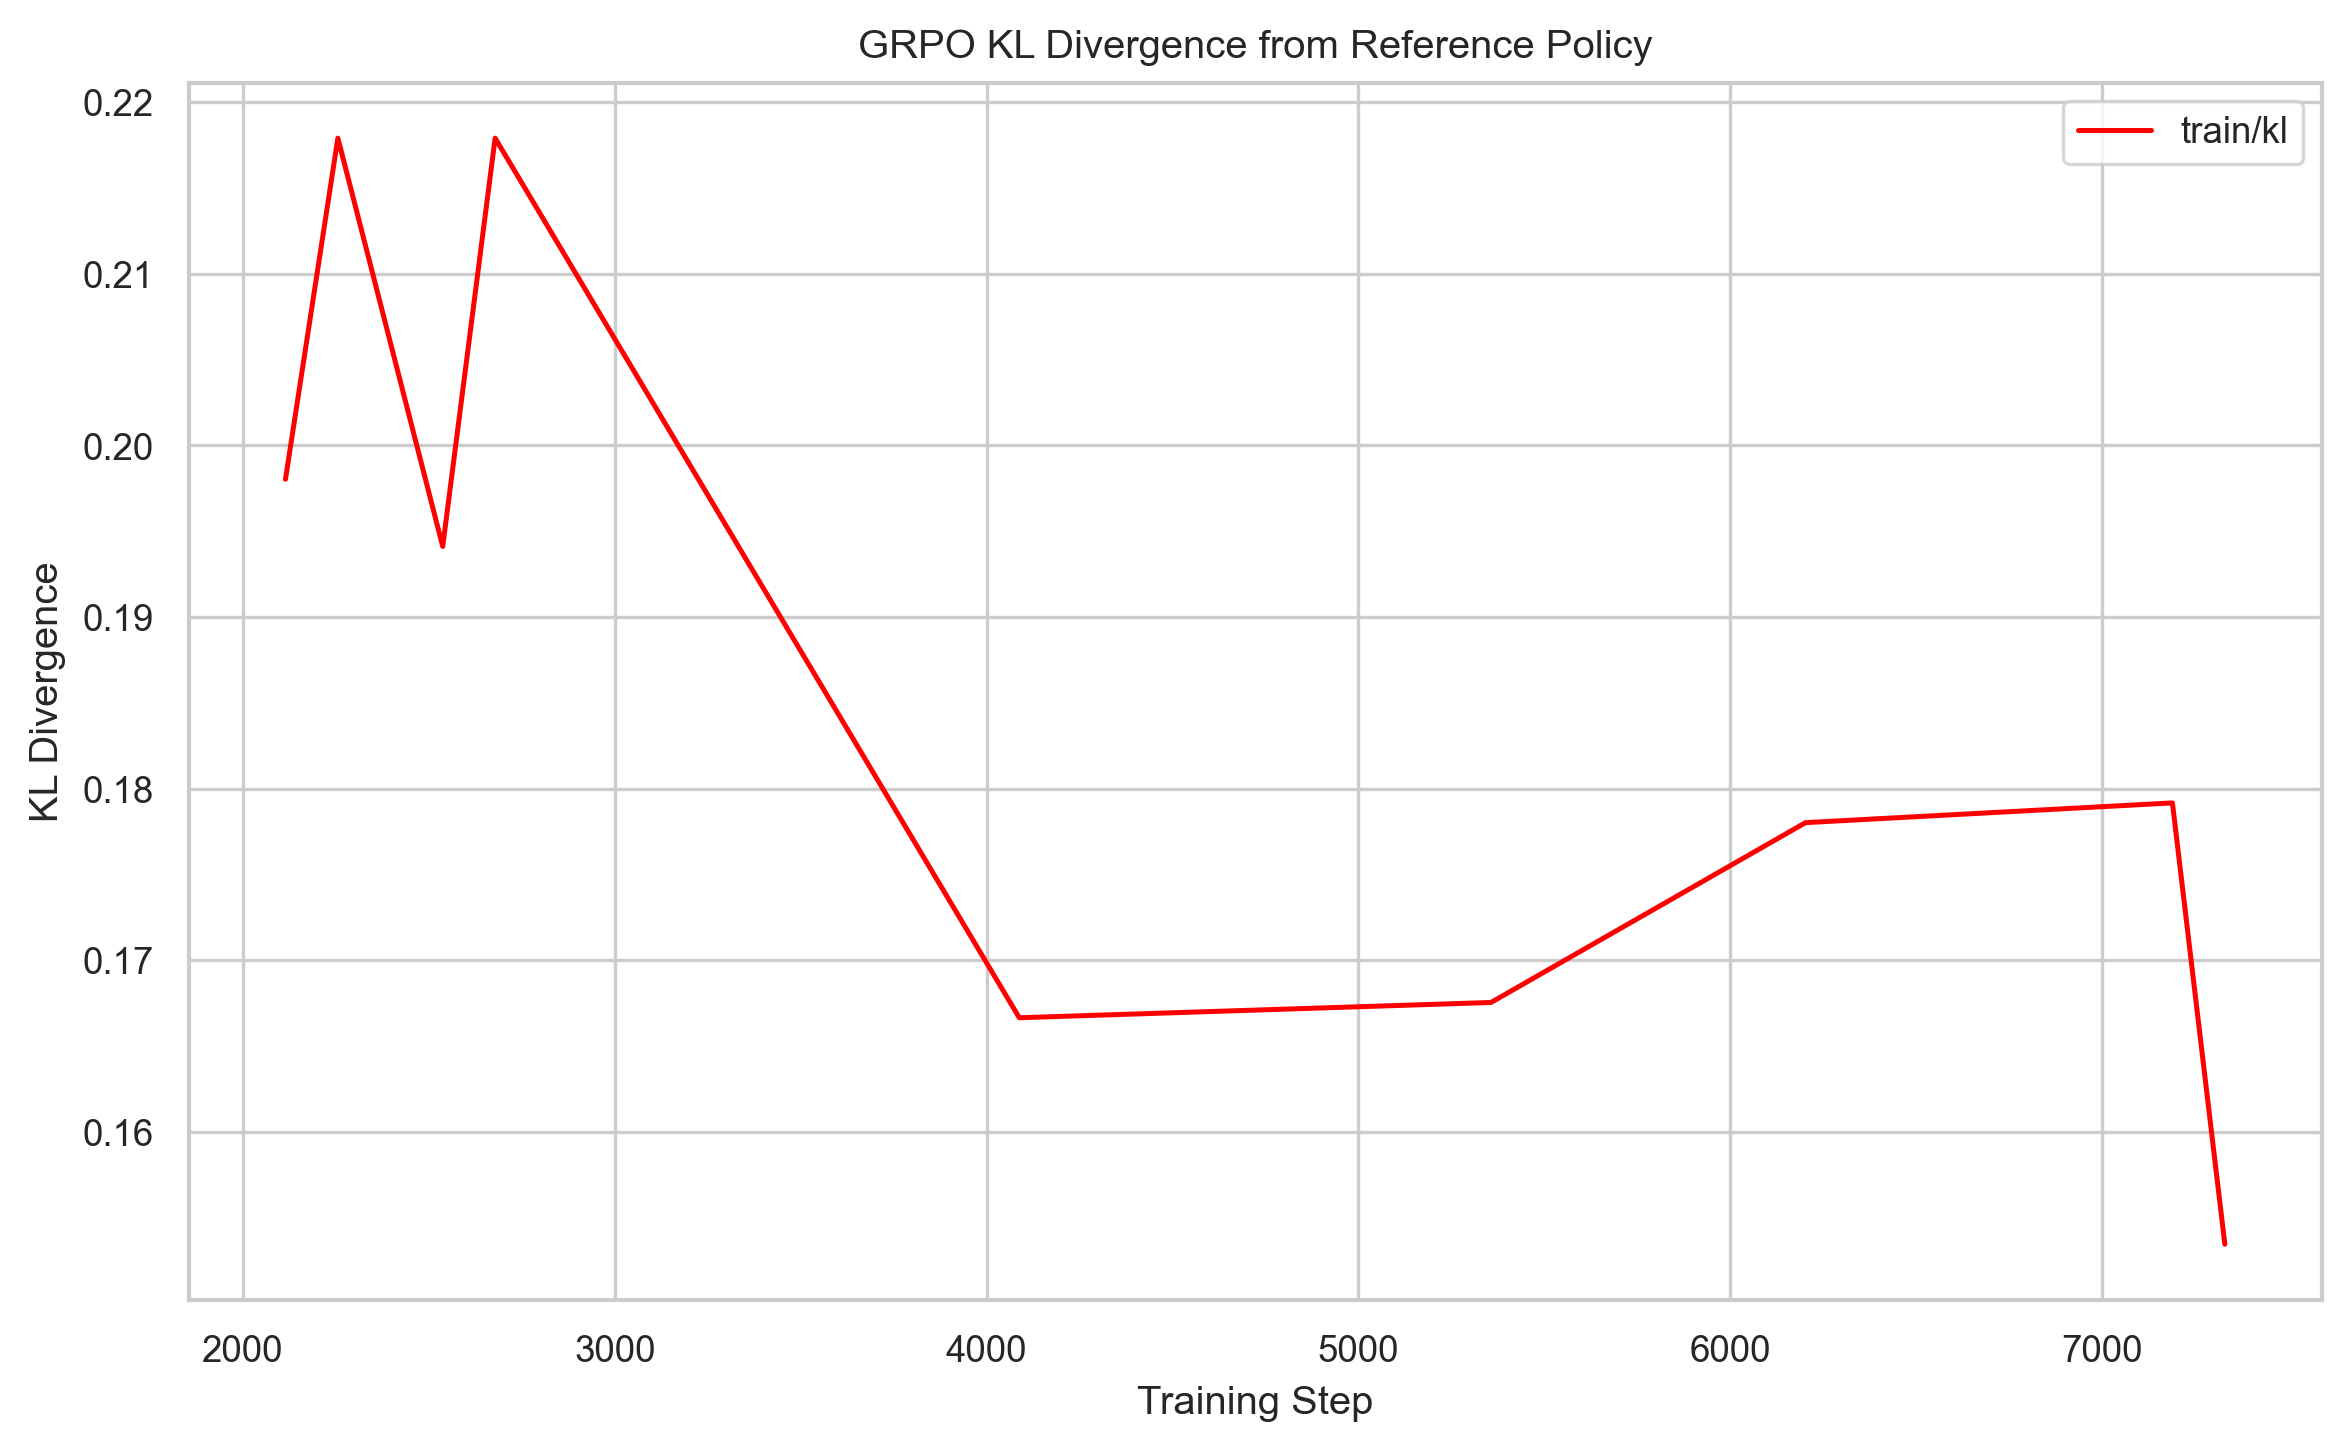
\includegraphics[width=0.48\textwidth]{figures/kl_divergence.png}
\caption{Detailed GRPO training metrics: Programmatic Reward Convergence (left) and KL Divergence from the reference policy (right).}
\label{fig:grpo_details}
\end{figure}

\section{Appendix: Prompts and Reward Functions}
\raggedbottom

\subsection{System Prompt Schema}
The following system prompt was used to enforce the structured generation scheme during GRPO training and inference:
\begin{verbatim}
You are a helpful assistant.
Given a question, you must decide whether it is ambiguous or not.
Output MUST follow this format:
Action: Clarify|Answer
Reasoning: <your reasoning>
Facets: <list of facets if ambiguous, else empty>
Response: <clarifying question or direct answer>
\end{verbatim}

\subsection{Programmatic Reward Functions}
Below is a simplified snippet of the deterministic Python validation scripts used to compute $\mathcal{R}_{\text{format}}$ and $\mathcal{R}_{\text{routing}}$ during GRPO training:

\begin{verbatim}
def format_reward_func(prompts, completions, **kwargs):
    """Reward function that checks for the exact format constraints."""
    rewards = []
    for completion in completions:
        text = completion[0]["content"] if isinstance(completion, list) else completion
        has_action = "Action:" in text
        has_reasoning = "Reasoning:" in text
        has_facets = "Facets:" in text
        has_response = "Response:" in text

        if has_action and has_reasoning and has_facets and has_response:
            rewards.append(1.0)
        else:
            rewards.append(-1.0)
    return rewards

def action_reward_func(prompts, completions, **kwargs):
    """Reward function that checks if the predicted action matches the target."""
    rewards = []
    target_actions = kwargs.get("target_action", [])

    for i, completion in enumerate(completions):
        text = completion[0]["content"] if isinstance(completion, list) else completion
        target = target_actions[i]

        action_match = re.search(r"Action:\s*(Clarify|Answer)", text)
        if action_match:
            pred_action = action_match.group(1)
            if pred_action == target:
                rewards.append(1.0)
            else:
                rewards.append(-1.0)
        else:
            rewards.append(-1.0)
    return rewards
\end{verbatim}

\section{Appendix: Training Hyperparameters}
\label{sec:hyperparams}
To ensure full reproducibility, we report the exact hyperparameters utilized during the Supervised Fine-Tuning (SFT), Direct Preference Optimization (DPO), and Group Relative Policy Optimization (GRPO) stages. Both stages utilized LoRA (Low-Rank Adaptation) injected into the attention and MLP modules. All experiments were conducted using the \texttt{transformers} and \texttt{trl} libraries, utilizing the Unsloth framework for efficient hardware acceleration via Triton kernels and Flash Attention. Models were trained on NVIDIA RTX A6000 and A100 GPUs using \texttt{bfloat16} precision.

\begin{table}[h]
\centering
\caption{Hyperparameters for Supervised Fine-Tuning (SFT)}
\begin{tabular}{lll}
\toprule
\textbf{Hyperparameter} & \textbf{Value} & \textbf{Description} \\
\midrule
Learning Rate & $2 \times 10^{-5}$ & Peak learning rate for the AdamW optimizer \\
Optimizer & AdamW & Using PyTorch's \texttt{adamw\_torch} implementation \\
Epochs & 3 & Number of passes over the training dataset \\
Per-Device Batch Size & 1 & Number of samples per forward pass per GPU \\
Gradient Accumulation & 8 & Steps to accumulate gradients before backward pass \\
Warmup Ratio & 0.05 & Fraction of steps used to linearly warmup the learning rate \\
Max Sequence Length & 2048 & Maximum context length in tokens \\
Precision & \texttt{bfloat16} & Used for both training and inference \\
\bottomrule
\end{tabular}
\label{tab:sft_hyperparams}
\end{table}

\begin{table}[h]
\centering
\caption{Hyperparameters for Direct Preference Optimization (DPO)}
\begin{tabular}{lll}
\toprule
\textbf{Hyperparameter} & \textbf{Value} & \textbf{Description} \\
\midrule
Learning Rate & $5 \times 10^{-7}$ & Drastically lowered to prevent SFT regression \\
KL Penalty ($\beta$) & 0.1 & Controls the constraint to the reference model \\
Optimizer & AdamW & Using PyTorch's \texttt{adamw\_torch} implementation \\
Epochs & 1 & Single pass over the preference dataset \\
Per-Device Batch Size & 1 & Number of samples per forward pass per GPU \\
Gradient Accumulation & 8 & Steps to accumulate gradients before backward pass \\
Warmup Ratio & 0.1 & Fraction of steps used to linearly warmup the learning rate \\
Max Prompt Length & 1024 & Maximum length for the input context \\
Max Sequence Length & 2048 & Maximum overall sequence length \\
Precision & \texttt{bfloat16} & Used for both training and inference \\
\bottomrule
\end{tabular}
\label{tab:dpo_hyperparams}
\end{table}

\begin{table}[h]
\centering
\caption{Hyperparameters for Group Relative Policy Optimization (GRPO)}
\begin{tabular}{lll}
\toprule
\textbf{Hyperparameter} & \textbf{Value} & \textbf{Description} \\
\midrule
Learning Rate & $5 \times 10^{-6}$ & Peak learning rate for RL optimization \\
KL Penalty ($\beta$) & 0.1 & Controls the constraint to the SFT reference model \\
Optimizer & AdamW & Using PyTorch's \texttt{adamw\_torch} implementation \\
Epochs & 1 & Single pass over the training dataset \\
Per-Device Batch Size & 1 & Number of samples per forward pass per GPU \\
Gradient Accumulation & 8 & Steps to accumulate gradients before backward pass \\
Warmup Ratio & 0.1 & Fraction of steps used to linearly warmup the learning rate \\
Max Prompt Length & 512 & Maximum length for the input context \\
Max Completion Length & 512 & Maximum length for the generated rollout \\
Rollouts per Prompt ($G$) & 8 & Number of generations sampled per input for group advantage \\
Precision & \texttt{bfloat16} & Used for both training and inference \\
\bottomrule
\end{tabular}
\label{tab:grpo_hyperparams}
\end{table}

\section{Appendix: Comprehensive Evaluation Leaderboard}
\label{sec:appendix_full_eval}
To provide a complete picture of the optimization landscape, Table \ref{tab:full_eval} details the comprehensive LLM-as-a-Judge evaluation results for all primary pipelines and extended ablation baselines.

\begin{table*}[!ht]
  \caption{Comprehensive LLM-as-a-Judge Evaluation Leaderboard across all computed metrics.}
  \label{tab:full_eval}
  \begin{center}
    \begin{small}
      \begin{sc}
        \begin{tabular}{lcccccc}
          \toprule
          Metric & Base & DPO Only & SFT & SFT $\rightarrow$ DPO & ORPO & SFT $\rightarrow$ GRPO \\
          \midrule
          Ambiguity Detection & 0.966 & 0.944 & 0.970 & 0.972 & 0.972 & 0.948 \\
          Clarification Quality & 0.784 & 0.784 & 0.796 & 0.796 & 0.796 & 0.798 \\
          Usefulness & 0.880 & 0.880 & 0.896 & 0.898 & 0.896 & 0.898 \\
          Model Accuracy & 0.620 & 0.600 & 0.640 & 0.620 & 0.640 & 0.640 \\
          Clarify Precision & 0.617 & 0.604 & 0.658 & 0.657 & 0.636 & 0.643 \\
          Clarify Recall & 0.967 & 0.967 & 0.833 & 0.767 & 0.933 & 0.900 \\
          Clarify F1 & 0.753 & 0.744 & 0.735 & 0.708 & 0.757 & 0.750 \\
          Action F1 (Answer) & 0.174 & 0.091 & 0.438 & 0.457 & 0.308 & 0.357 \\
          Macro F1 & 0.464 & 0.417 & 0.586 & 0.582 & 0.532 & 0.554 \\
          Answer Accuracy & 0.050 & 0.050 & 0.050 & 0.000 & 0.100 & 0.100 \\
          Facet Generation Rate & 0.085 & 0.083 & 1.000 & 1.000 & 0.932 & 1.000 \\
          Clarify Ratio & 1.567 & 1.600 & 1.267 & 1.167 & 1.467 & 1.400 \\
          \bottomrule
        \end{tabular}
      \end{sc}
    \end{small}
  \end{center}
\end{table*}

%%%%%%%%%%%%%%%%%%%%%%%%%%%%%%%%%%%%%%%%%%%%%%%%%%%%%%%%%%%%%%%%%%%%%%%%%%%%%%%
%%%%%%%%%%%%%%%%%%%%%%%%%%%%%%%%%%%%%%%%%%%%%%%%%%%%%%%%%%%%%%%%%%%%%%%%%%%%%%%

\end{document}

% This document was modified from the file originally made available by
% Pat Langley and Andrea Danyluk for ICML-2K. This version was created
% by Iain Murray in 2018, and modified by Alexandre Bouchard in
% 2019 and 2021 and by Csaba Szepesvari, Gang Niu and Sivan Sabato in 2022.
% Modified again in 2023 and 2024 by Sivan Sabato and Jonathan Scarlett.
% Previous contributors include Dan Roy, Lise Getoor and Tobias
% Scheffer, which was slightly modified from the 2010 version by
% Thorsten Joachims & Johannes Fuernkranz, slightly modified from the
% 2009 version by Kiri Wagstaff and Sam Roweis's 2008 version, which is
% slightly modified from Prasad Tadepalli's 2007 version which is a
% lightly changed version of the previous year's version by Andrew
% Moore, which was in turn edited from those of Kristian Kersting and
% Codrina Lauth. Alex Smola contributed to the algorithmic style files.
